% Created 2016-10-08 六 23:08
\documentclass[11pt]{article}
\usepackage[utf8]{inputenc}
\usepackage[T1]{fontenc}
\usepackage{fixltx2e}
\usepackage{graphicx}
\usepackage{longtable}
\usepackage{float}
\usepackage{wrapfig}
\usepackage{soul}
\usepackage{textcomp}
\usepackage{marvosym}
\usepackage{wasysym}
\usepackage{latexsym}
\usepackage{amssymb}
\usepackage{hyperref}
\tolerance=1000
\providecommand{\alert}[1]{\textbf{#1}}

\title{fast-rcnn}
\author{shhs}
\date{\today}
\hypersetup{
  pdfkeywords={},
  pdfsubject={},
  pdfcreator={Emacs Org-mode version 7.9.3f}}

\begin{document}

\maketitle

\setcounter{tocdepth}{3}
\tableofcontents
\vspace*{1cm}

\section{Fast R-CNN --Ross Girshick}
\label{sec-1}

 
Paper: \href{http://arxiv.org/abs/1504.08083}{Fast R-CNN}
Code: \href{https://github.com/rbgirshick/fast-rcnn}{Fast R-CNN's code}
\subsection{Fast R-CNN architecture and training}
\label{sec-1-1}


   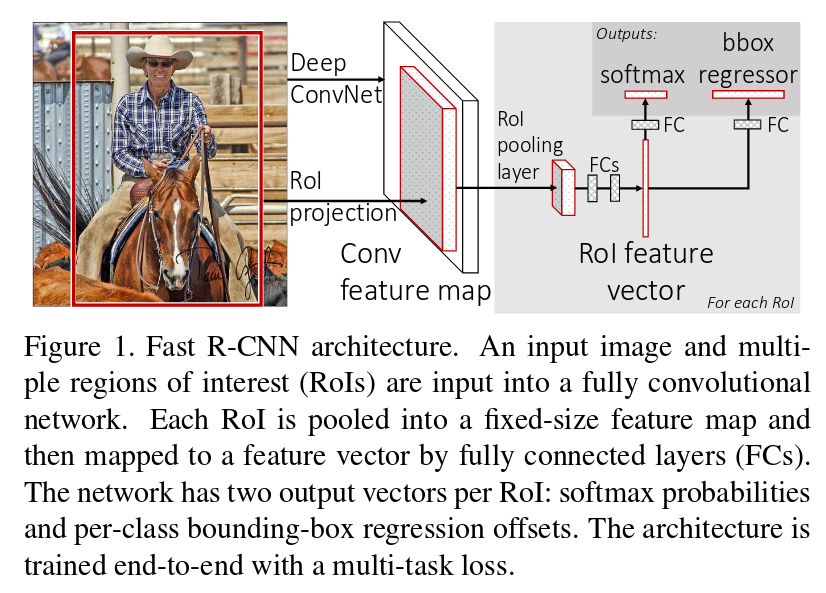
\includegraphics[width=.9\linewidth]{./pic_fast_rcnn/1.png}
\begin{itemize}
\item inputs: \textbf{an entire image}, \textbf{a set of object proposals}
\item several convolutional and max pooling layers -> produce a conv feature map
\item for each object proposal: a RoI(region of interest) pooling layer extracts a 
     fixed-length feature vector from the feature map
\item each feature vector is fed into a sequence of fully connected(fc) layers 
     that finally branch into two sibling(兄弟,姐妹,同属) output layers:
     \textbf{one} that produces softmax probability estimates over K object classes
     plus a catch-all ``background'' class and \textbf{another layer} that outputs 
     four real-valued numbers for each of the K object classes.
\item $\Box$ ? 2. \emph{Each set of 4 values encodes refined bounding-box positions for one of            the K classes.}
\end{itemize}
\subsubsection{The RoI pooling layer}
\label{sec-1-1-1}

\begin{itemize}
\item The RoI pooling layer uses max pooling to convert the features inside any valid
\end{itemize}
    region of interest into a small feature map with a fixed spatial extent of HxW,
    wherer H and W are layer hyper-parameters that are independent of any particular RoI.

\begin{itemize}
\item RoI: (r,c,h,w) specifies its top-left corner(r,c) and its height and width(h,w).
\item RoI max pooling layer divides the hxw RoI window into an HxW grid of sub-windows of
      approximate size h/H x w/W and then max-pooling the values in each sub-window into 
      the corresponding output grid cell.
\end{itemize}
\subsubsection{Initializing from pre-trained networks}
\label{sec-1-1-2}


\begin{itemize}
\item When a pre-trained network initializes a Fast R-CNN network, it undergoes three
      transformations:
\begin{enumerate}
\item The last max pooling layer is replaced by a RoI pooling layer that is configured
         by setting H and W to be compatible with the net's first fully connected layer
         (e.g., H = W = 7 for VGG16).
\item The network's last fully connected layer and softmax are replaced with the two 
         sibling layers described earlier: a fully connected layer and softmax over K + 1
         categories, category-specific bounding-box regressors.
\item The network is modified to take two data inputs: a list of images and a list of
         RoIs in those images.
\end{enumerate}
\end{itemize}
\subsubsection{Fine-tuning for detection}
\label{sec-1-1-3}


\begin{itemize}
\item In Fast R-CNN training, stochastic gradient descent(SGD) mini-batches are sampled 
      hierarchically.
\begin{enumerate}
\item First sampling N images
\item Second sampling R/N RoIs from each image.
\end{enumerate}
\item RoIs from the same image share computation and memory in the forward and backward
      passes.
\item One concern over this strategy is it may cause slow training convergence because
      RoIs from the same image are correlated. This concern does not appear to be a 
      practical issue and we achieve good results with N = 2 and R = 128 using fewer
      SGD iterations than R-CNN.
\end{itemize}
\begin{itemize}

\item Multi-task loss\\
\label{sec-1-1-3-1}%
\begin{itemize}
\item A Fast R-CNN network has two sibling output layers.
\begin{enumerate}
\item The first outputs a discrete probability distribution(per RoI), 
          $p = (p_0, ..., p_K)$, over K + 1 categories.(a softmax over the K + 1 outputs of a
          fully connected layer.
\item The second sibling layer outputs bounding-box regression offsets, 
          $t^k = (t_x^k, t_y^k, t_w^k, t_h^k)$, for each of the K object classes, indexed by k.
\item $\Box$ We use the parameterization for $t^k$ given in \footnote{R. Girshick, J. Donahue, T. Darrell, and J. Malik.  
  Rich feature hierarchies for accurate object detection and semantic segmentation. In CVPR, 2014.
 }, in which t$^k$ specifies a
          scale-invariant translation and log-space height/width shift relative to an object 
          proposal.
\end{enumerate}
\item \textbf{Each trainging RoI} is labeled with a ground-truth class u and a ground-truth bounding-box
       regression target v. We use a multi-task loss L on each labeled RoI to jointly train for
       classification and bounding-box regression:
       \begin{equation}
         L(p, u, t^u, v) = L_{cls}(p, u) + \lambda[u\ge1]L_{loc}(t^u, v)         
       \end{equation}
       in which $L_{cls}(p, u)  = -logp_u$ is log loss for true class u.
\item The second task loss , $L_loc$, is defined over a tuple of true bounding-box regression 
       targets for class u. The Iverson bracket indicator function $[u\ge1]$ evaluates to 1 when 
       $u>1$ and 0 otherwise.For background RoIs there is no notion of a ground-truth bounding box
       and hence $L_{loc}$ is ignored. For bounding-box regression, we use the loss
       \begin{equation}
         L_{loc}(t^u, v) = \sum_{i\in{x, y, w, h}} smooth_{L_1}(t_i^u - v_i)         
       \end{equation}
       in which 
       \begin{equation}
         smooth_{L_1}(x) = 
       \begin{cases}
       {0.5x^2} &\mbox{if |x| < 1}\\
       {|x| - 0.5} &\mbox{otherwise}
       \end{cases}
       \end{equation}
       is a robust $L_1$ loss that is less sensitive to outliers than the $L_2$ loss used in 
       R-CNN and SPPnet.
\begin{itemize}
\item When the regression targets are unbounded, training with $L_2$ loss can require careful
         tuning of learning rates in order to prevent exploding gradients. Eq.3 eliminates this
         sensitivity.
\end{itemize}
\item We normalize the ground-truth regression targets $v_i$ to have zero mean and unit variance.
       All experiments use $\lambda = 1$.
\item \footnote{D. Erhan, C. Szegedy, A. Toshev, and D. Anguelov. 
Scalable object detection using deep neural networks. In CVPR, 2014.
 } uses a related loss to train a class agnostic object proposal network. \footnotemark[2] advocates
       for a two-network system that separates localization and classification.
\item OverFeat\footnote{P. Sermanet,  D. Eigen,  X. Zhang,  M. Mathieu,  R. Fergus,and Y. LeCun.  
OverFeat: Integrated Recognition, Localization and Detection using Convolutional Networks.  
In ICLR,2014.
 }, R-CNN\footnotemark[1], and SPPnet\footnote{K. He, X. Zhang, S. Ren, and J. Sun. 
Spatial pyramid pooling in  deep  convolutional  networks  for  visual  recognition.   
In ECCV, 2014.
 } alse train classifiers and bounding-box 
       localizers, however these methods use stage-wise training, which we show is suboptimal
       for Fast R-CNN.
\end{itemize}


\item Mini-batch sampling\\
\label{sec-1-1-3-2}%
\begin{enumerate}
\item During fine-tuning, each SGD mini-batch is constructed from N = 2 images, chosen uniformly
        at random. We use mini-batches of size R = 128, sampling 64 RoIs from each images.
\item As in \footnotemark[1], we take 25\% of the RoIs from object proposals that have intersection over
        union(IoU) overlap with a ground-truth bounding box of at least 0.5. These RoIs comprise
        the examples labeled with a foreground object class, i.e. $u \ge 1$.
\item The remaining RoIs are sampled from object proposals that have a maximum IoU with ground truth
        in the interval [0.1, 0.5), following \footnotemark[4].
\begin{enumerate}
\item These are the background examples and are labeled with u = 0.
\item The lower threshold of 0.1 appears to act as a heuristic for hard example mining \footnote{P.  Felzenszwalb,  R.  Girshick,  D.  McAllester,  and  D.  Ramanan.   
Object detection with discriminatively trained part based models.
TPAMI, 2010.
 }.
\end{enumerate}
\item During traing, images are horizontally flipped with probability 0.5. No other data 
        augmentation is used.
\end{enumerate}


\item Back-propagation through RoI pooling layers\\
\label{sec-1-1-3-3}%
\begin{enumerate}
\item The RoI pooling layer's backwards function computes partial derivative of the loss
        function with respect to each input variable $x_i$ by following the argmax switches:
        \begin{equation}
          \frac{\partial{L}}{\partial{x_i}} = \sum_r\sum_j[i = i*(r,j)]\frac{\partial{L}}{\partial{y_{rj}}}
        \end{equation}
\begin{itemize}
\item where $x_i\in{R}$ be the i-th activation input into the RoI pooling layer and
\end{itemize}
$y_{rj}$ be the layer's j-th output from the r-th RoI.
\begin{itemize}
\item The RoI pooling layer computes $y_{rj}=x_{i*(r,j)}$, in which $i*(r,j)=argmax_{i^{'}\in{R(r,j)}}x_{i^{'}}$.
\end{itemize}
$R(r,j)$ is the index set of inputs in the sub-window over which the output unit $y_{rj}$ 
        max pools.
\end{enumerate}


\item SGD hyper-parameters\\
\label{sec-1-1-3-4}%
\begin{itemize}
\item The fully connected layers used for softmax classification and bounding-box regression
       are initialized from $N(0,0.01^2)$ and $N(0,0.001^2)$. Biases are initialized to 0.
\item All layers use a pre-layer learning rate of 1 for weights and 2 for biases and a global
       learning rate of 0.001.
\item When training on VOC07 or VOC12 trainval we run SGD for 30k mini-batch iterations, and
       then lower the learning rate to 0.0001 and train for another 10k iterations.
\item Momentum : 0.9 , Parameter decay : 0.0005(on weights and biases)
\end{itemize}

\end{itemize} % ends low level
\subsubsection{Scale invariance}
\label{sec-1-1-4}


\begin{enumerate}
\item We explore two ways of achieving scale invariant object detection:
\begin{enumerate}
\item via ``brute force''
\item by using image pyramids
\end{enumerate}
\item These strategies follow the two approaches in \footnotemark[4].
\item Brute-force approach
\begin{itemize}
\item Each image is processed at a pre-defined pixel size during both training and testing.
\item The network must directly learn scale-invariant object detection from the training data.
\end{itemize}
\item Multi-scale approach
\begin{itemize}
\item Provides approximate scale-invariance to the network through an image pyramid.
\item At test-time, the image pyramid is used to approximately scale-normalize each object 
         proposal.
\item During multi-scale training, we randomly sample a pyramid scale each time an image is
         sampled, following \footnotemark[4], as a form of data augmentation.
\end{itemize}
\item We experiment with multi-scale training for smaller networks only, due to GPU memory limits.
\end{enumerate}
          
\subsection{Fast R-CNN detection}
\label{sec-1-2}


\begin{itemize}
\item The network takes as input an image(or an image pyramid, encoded as a list of images) and a list
     of R object proposals to score. At test-time, R is typically around 2000, although we will 
     consider cases in which it is larger($\approx45k$).
\item When using an image pyramid, each RoI is assigned to the scale such that the scaled RoI is
     closest to $224^2$ pixels in area \footnotemark[4].
\item For each test RoI r, the forward pass outputs a class posterior probability distribution p and
     a set of predicted bounding-box offsets relative to r(each of the K classes gets its own refined
     bounding-box prediction).
\item We assign a detection confidence to r for each object class k using the estimated probability 
     $P_r(class=k|r)=p_k$.
\item We then perform non-maximum suppression independently for each class using the algorithm and 
     settings from R-CNN\footnotemark[1].
\end{itemize}
\subsubsection{Truncated SVD for faster detection}
\label{sec-1-2-1}


   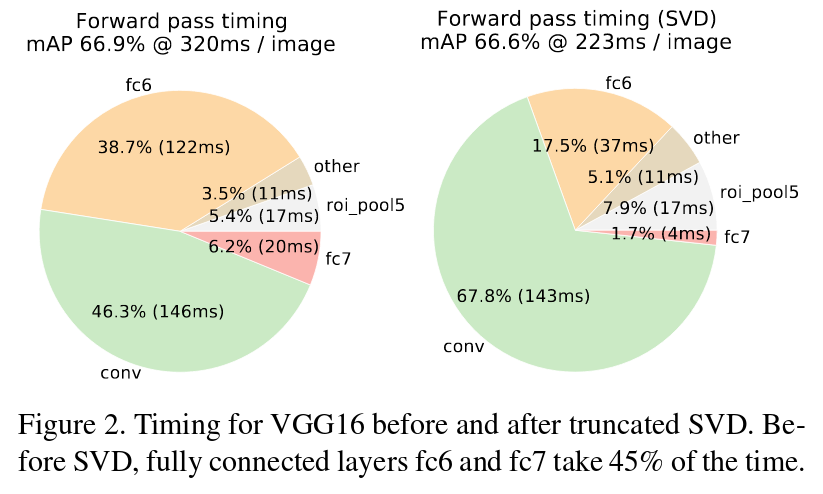
\includegraphics[width=.9\linewidth]{./pic_fast_rcnn/2.png}
\begin{itemize}
\item For whole-image classification, the time spent computing the fully connected layers is small 
     compared to the conv layers. On the contrary, for detection the number of RoIs to process is
     large and nearly half of the forward pass time is spent computing the fully connected layers.
\item Large fully connected layers are easily accelerated by compressing them with truncated 
     SVD\footnote{E. Denton, W. Zaremba, J. Bruna, Y. LeCun, and R. Fergus.
Exploiting linear structure within convolutional networks for efficient evaluation. 
InNIPS, 2014.
 }\textsuperscript{,}\,\footnote{J.  Xue,  J.  Li,  and  Y.  Gong.   
Restructuring  of  deep  neural network acoustic models with singular value decomposition.
In Interspeech, 2013.
 }.
\item In this technique, a layer parameterized by the $u\times{v}$ weight matrix W is approximately 
     factorized as
     \begin{equation}
       W\approx{U\sum_tV^T}
     \end{equation}
     In this factorization, U is a $u\times{t}$ matrix comprising the first t left-singular vectors
     of W, $\sum_t$ is a $t\times{t}$ diagonal matrix containing the top t singular values of W,
     and V is $v\times{t}$ matrix comprising the first t right-singular vectors of W.
\item Truncated SVD reduces the parameter count from $uv$ to $t(u+v)$, which can be 
     significant if t is much smaller than min(u,v).
\item To compress a network, the single fully connected layer corresponding to W is replaced
     by two fully connected layers, without a non-linearity between them.
\begin{enumerate}
\item The first of these layers uses the weight matrix $\sum_tV^T$ (and no biases).
\item The second uses $U$ (with the original biases associated with $W$).
\end{enumerate}
\item This simple compression method gives good speedups when the number of RoIs is large.
\end{itemize}
     
\subsection{Main results}
\label{sec-1-3}


\begin{itemize}
\item Three main results support this paper's contributions:
\begin{enumerate}
\item State-of-the-art mAP on VOC07, 2010, and 2012
\item Fast training and testing compared to R-CNN, SPPnet
\item Fine-tuning conv layers in VGG16 improves mAP
\end{enumerate}
\end{itemize}
\subsubsection{Experimental setup}
\label{sec-1-3-1}

\begin{itemize}
\item Our experiments use three pre-trained ImageNet models that are available online\footnote{https://github.com/BVLC/caffe/wiki/Model-Zoo
 }.
\begin{enumerate}
\item The first is the CaffeNet(essentially AlexNet\footnote{A. Krizhevsky, I. Sutskever, and G. Hinton.  
ImageNet classification with deep convolutional neural networks. 
In NIPS,2012.
 }) from R-CNN\footnotemark[1]. We alternatively
         refer to this CaffeNet as model $S$, for ``small''.
\item The second network is VGG$_{\mathrm{CNN}}$$_M$$_{\mathrm{1024}}$ from \footnote{K. Chatfield, K. Simonyan, A. Vedaldi, and A. Zisserman.
Return of the devil in the details:  Delving deep into convolutional nets. 
In BMVC, 2014.
 }, which has the same depth as $S$,
         but is wider. We call this network model $M$, for ``medium''.
\item The final network is the very deep VGG16 model from \footnote{K.  Simonyan  and  A.  Zisserman.   
Very  deep  convolutional networks for large-scale image recognition.  
In ICLR, 2015.
 }. We call  it model $L$.
\end{enumerate}
\item In this section, all experiments use single-scale training and testing(s=600).
\end{itemize}
\subsubsection{VOC 2010 and 2012 results}
\label{sec-1-3-2}

    
\subsubsection{VOC 2007 results}
\label{sec-1-3-3}
\subsubsection{Training and testing time}
\label{sec-1-3-4}


\begin{itemize}
\item Fast training  and testing times are our second main result.

      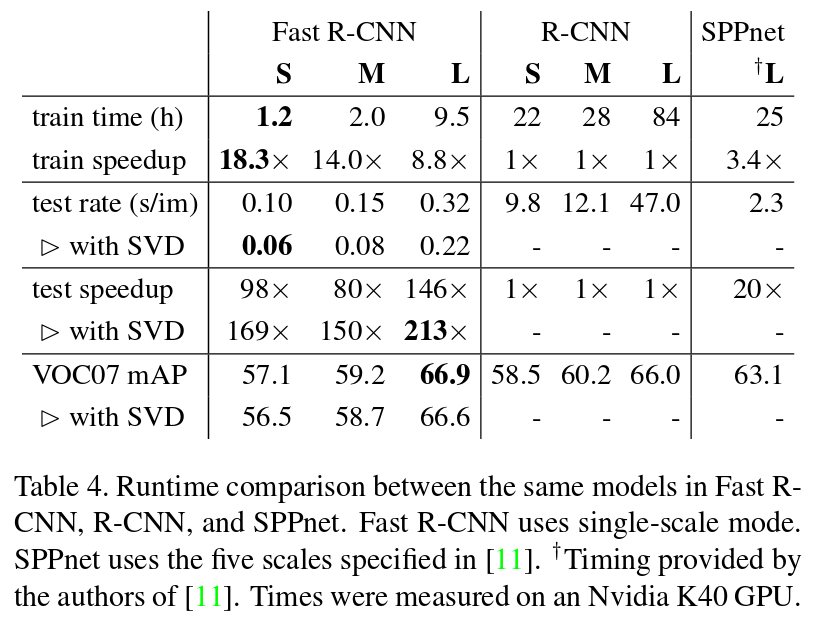
\includegraphics[width=.9\linewidth]{./pic_fast_rcnn/table4.png}
\end{itemize}
\begin{itemize}

\item Truncated SVD\\
\label{sec-1-3-4-1}%
\begin{itemize}
\item Truncated SVD can reduce detection time by more than 30\% with only a small drop 
       in mAP and without needing to perform additional fine-tuning after model compression.
\item Using the top 1024 singular values from the $25088\times{4096}$ matrix in VGG16's fc6 layer
       and the top 256 singular values from the $4096\times{4096}$ fc7 layer reduces runtime
       with little loss in mAP.

       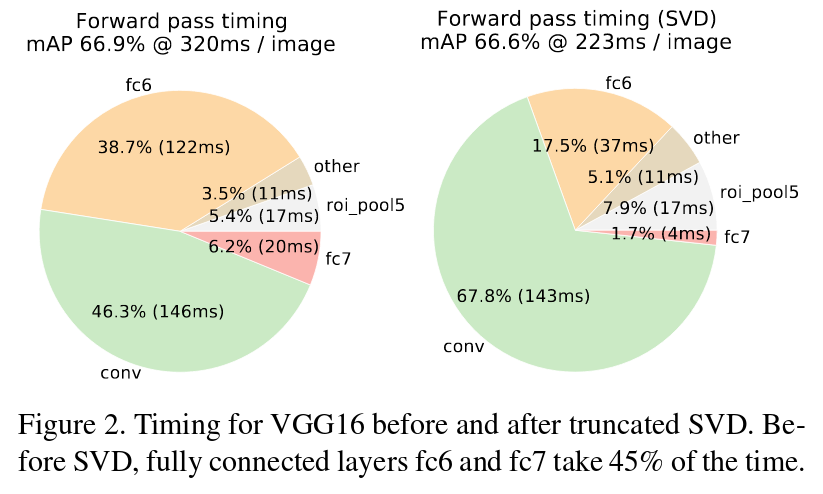
\includegraphics[width=.9\linewidth]{./pic_fast_rcnn/2.png}
\end{itemize}


\end{itemize} % ends low level
\subsubsection{Which layers to fine-tune?}
\label{sec-1-3-5}


\begin{itemize}
\item Our hypothesis: training through the RoI pooling layer is important for very deep nets.

      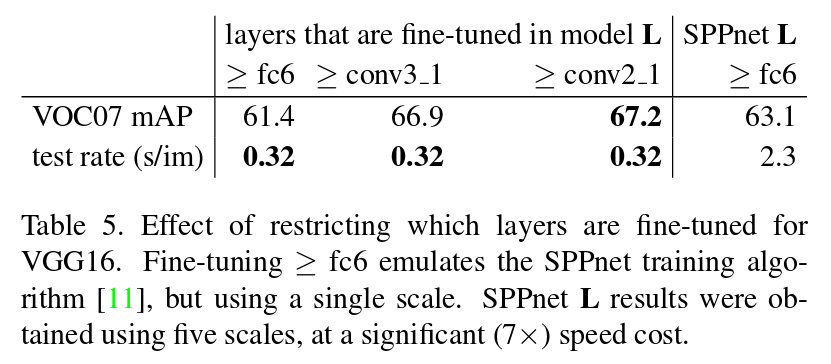
\includegraphics[width=.9\linewidth]{./pic_fast_rcnn/table5.png}
\item Does this mean that all conv layers should be fine-tuned?
      In short, no.
\begin{enumerate}
\item In the smaller networks $S$ and $M$ , we find that conv1 is generic and task 
         independent(a well-known fact)\footnote{A. Krizhevsky, I. Sutskever, and G. Hinton.  
ImageNet classification with deep convolutional neural networks. 
In NIPS,2012.
 }. Allowing conv1 to learn, or not, has no
         meaningful effect on mAP.
\item For VGG16, we found it only necessary to update layers from conv3$_1$ and up(9 of the 13
         conv layers).
\item This observation is pragmatic:
\begin{enumerate}
\item updating from conv2$_1$ slows trainging by 1.3x (12.5 vs. 9.5 hours) compared to 
            learning from conv3$_1$
\item Updating from conv1$_1$ over-runs GPU memory
\end{enumerate}
\item All Fast R-CNN results in this paper using VGG16 fine-tune layers conv3$_1$ and up;
         all experiments with models $S$ and $M$ fine-tune layers conv3 and up.
\end{enumerate}
\end{itemize}
         
\subsection{Design evaluation}
\label{sec-1-4}


\begin{itemize}
\item We conducted experiments to understand how Fast R-CNN compares to R-CNN and SPPnet, as well 
     as to evaluate design decisions.
\end{itemize}
   
\subsubsection{Does multi-task training help?}
\label{sec-1-4-1}


\begin{itemize}
\item We observe that multi-task training improves pure classification accuracy relative to
      training for classification alone.
\item Stage-wise training improves mAP over column one, but underperforms multi-task training.
    
      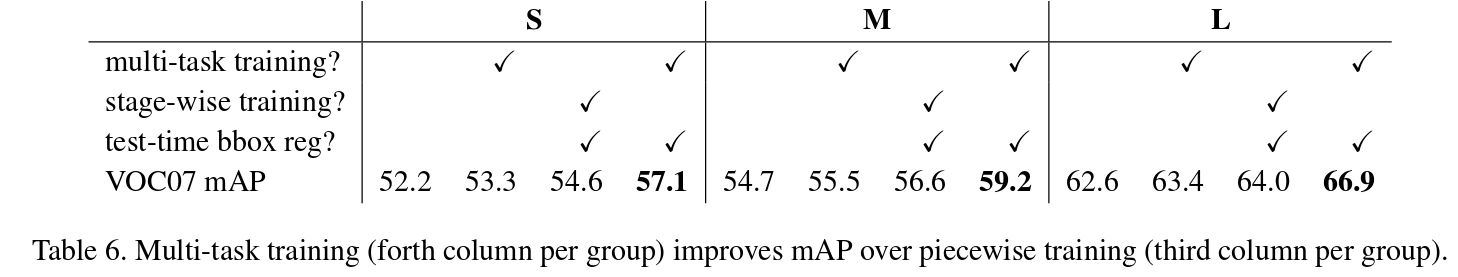
\includegraphics[width=.9\linewidth]{./pic_fast_rcnn/table6.png}
\end{itemize}
\subsubsection{Scale invariance : to brute force or finesse?}
\label{sec-1-4-2}


\begin{itemize}
\item We compare two strategies for achieving scale-invariant object detection:
      brute-force learning(single scale) and image pyramids(multi-scale). In either
      case, we define the scale s of an image to be the length of its shortest side.
\item All single-scale experiments use s = 600 pixels.
\item In the multi-scale setting, we use the same five scales specified in \footnotemark[4]
      $s\in{{480,576,688,864,1200}}$ to facilitate comparison with SPPnet.
      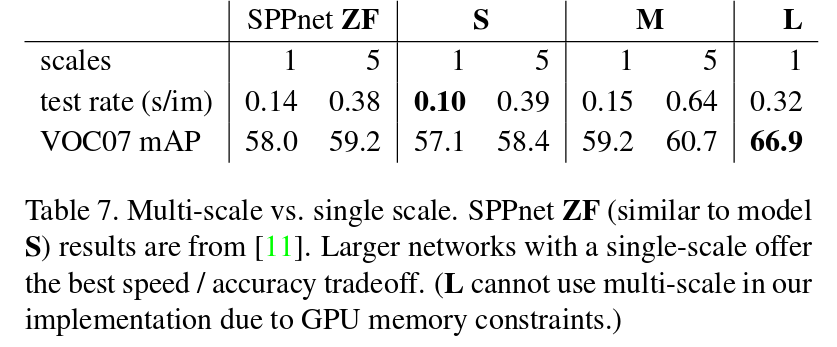
\includegraphics[width=.9\linewidth]{./pic_fast_rcnn/table7.png}
\item Deep ConvNets are adept at directly learning scale invariance.
\item The multi-scale approach offers only a small increase in mAP at a large cost
      in compute time.
\end{itemize}
\subsubsection{Do we need more training data?}
\label{sec-1-4-3}
\subsubsection{Do SVMs outperform softmax?}
\label{sec-1-4-4}


\begin{itemize}
\item Fast R-CNN uses the softmax classifier learnt during fine-tuning instead of
      training one-vs-rest linear SVMs post-hoc, as was done in R-CNN and SPPnet.
      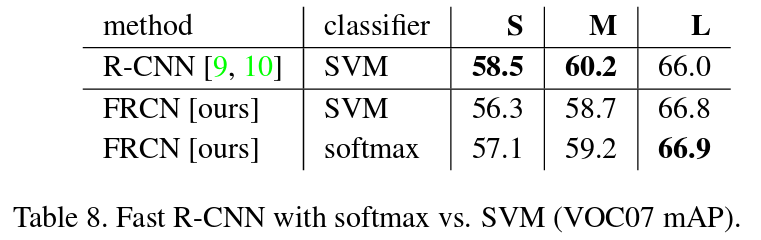
\includegraphics[width=.9\linewidth]{./pic_fast_rcnn/table8.png}
\item Softmax slightly outperforming SVM for all three networks.
\item This effect is small, but it demonstrates that ``one-shot'' fine-tuning is sufficient
      compared to previous multi-stage training approaches.
\item We note that softmax, unlike one-vs-rest SVMs, introduces competition between classes
      when scoring a RoI.
\end{itemize}
\subsubsection{Are more proposals always better?}
\label{sec-1-4-5}


\begin{itemize}
\item There are two types of object detectors : those that use a sparse set of object 
      proposals\footnote{J. Uijlings, K. van de Sande, T. Gevers, and A. Smeulders.
Selective search for object recognition.
IJCV, 2013.
 } and those that use a dense set DPM\footnote{P.  Felzenszwalb,  R.  Girshick,  D.  McAllester,  and  D.  Ramanan.   
Object detection with discriminatively trained part based models.
TPAMI, 2010.
 }.
\end{itemize}
\subsubsection{Preliminary MS COCO results}
\label{sec-1-4-6}
\subsection{Conclusion}
\label{sec-1-5}


\begin{itemize}
\item This paper proposes Fast R-CNN, a clean and fast update to R-CNN and SPPnet.
\item Of particular note, sparse object proposals appear to improve detector quality.
\item There may exist yet undiscovered techniques that allow dense boxes to perform 
     as well as sparse proposals.
\end{itemize}

\end{document}
